\documentclass[11pt]{exam}
\usepackage[margin=1in]{geometry}
\pagestyle{plain}
\usepackage{amsmath,amsfonts,amssymb,amsthm,enumerate}
\usepackage{multicol}
\usepackage[]{graphicx}
\usepackage{hyperref}
\usepackage{tikz}
\usepackage{pgfplots}
\usepackage{subfigure}
\usepackage[final]{pdfpages}

\addtolength{\footskip}{2\baselineskip} % to lower the page numbers
\title{\vspace{-0.5in} Math 115 \\ Worksheet Section 4.5}
\date{}


% \theoremstyle{definition}
% \newtheorem{problem}{Problem}
\renewcommand{\questionlabel}{\textbf{Problem~\thequestion.}}
% \printanswers

\begin{document}
\maketitle
\vspace{-0.75in}
\section*{Warm-up questions}
The {\bf cost function} $C(q)$ gives the cost of producing a quantity $q$ of a certain good.

\noindent
The {\bf revenue function} $R(q)$ gives the revenue received from selling a quantity $q$ of some good.

\noindent
The {\bf profit} $\pi(q)=$\fillin[\(R(q)-C(q)\)] gives the total profit from producing and selling $q$ of that good.

\noindent
To decide whether a company's profit would increase or decrease if the company increased or decreased production of a certain good, we might look at the marginal cost and marginal revenue:

\vspace{0.5em}
The {\bf marginal cost} is given by $\textrm{MC}(q)= \fillin[C'(q)]\approx
\fillin[C(q+1)-C(q)]$

\vspace{0.5em}
The {\bf marginal revenue} is given by $\textrm{MR}(q)= \fillin[R'(q)
]\approx \fillin[R(q+1)-R(q)]$
\vspace{1em}

\noindent
When can maximum profit occur?
\begin{solution}
  Where marginal cost = marginal revenue, other critical points where
  MR or MC do not exist, and at endpoints
\end{solution}
\vspace{1em}

\noindent
How do we identify the fixed cost of producing a certain good?
\begin{solution}
  The value of \(C(0)\).
\end{solution}
\vspace{3em}
\begin{questions}
  \question The total cost of producing \(q\) items is approximated by
    $C(q) = 5000+2.4q$ and the total revenue of selling \(q\) items is
    approximated by $R(q) = 4q$, both in dollars.  Find the fixed
    cost, marginal cost per item, and the price at which this
    commodity is sold. 
    \begin{solution}
      \begin{itemize}
      \item Fixed cost is \(C(0) = \$5000\)
      \item Marginal cost is \(C'(q) = \$2.4\)/item
      \item The commodity is sold at \(R'(q) = \$4\)/item
      \end{itemize}
    \end{solution}
    \vspace{.7in}
  \question A car wash operator pays \$35,000 for a franchise, then spends \$10 per car wash, which costs the consumer \$15.  Find the cost, revenue, and profit functions.
    \begin{solution}
      \begin{itemize}
      \item The fixed cost is \(\$35,000\) and the cost of each wash is
      \(\$10\), so the cost of giving \(q\) car washes is \(C(q) = 35000+10q\)
      \item The revenue is \(\$15\) per car wash, so \(R(q) = 15q\)
      \item \(\pi(q) = R(q)-C(q) = 5q-35000\)
      \end{itemize}
    \end{solution}
    \vspace{.7in}
  \question Revenue of selling \(q\) items is given by $R(q)=450q$, and cost is given by $C(q)=$ 10,000 $ +\; 3q^2$.  At what quantity is profit maximized?  What is the total profit at this production level?
    \begin{solution}
      We first note that \(\pi(q) = R(q)-C(q) = -3q^2+450q-10000\) and
      so \(\pi'(q) = -6q+450\). We then find the critical points.
      \begin{itemize}
      \item \(\pi'(q) = 0\): at \(q = \frac{450}{6} = 125\)
      \item \(\pi'(q)\) DNE: none
      \end{itemize}
      Then, we check \(\pi(0) = -10000\), \(\pi(125) = -3 \cdot 125
      \cdot 125 + 450 \cdot 125 -10000 = 3 \cdot 125 \cdot 125 - 100
      \cdot 100 > 0\) and \(\lim_{q\to\infty}
      \pi(q) = -\infty\). Therefore, profit is maximized by selling
      \(125\) items with a profit of \(\pi(125)= \$36,875\).
    \end{solution}
    \vspace{0.7in}
  \question When production is \(q=2000\) units, marginal revenue is
    \$4 per unit and marginal cost is \$3.25 per unit.  Do you expect
    maximum profit to occur at a production level above or below 2000 units? Explain.
    \begin{solution}
      Above \(2000\) units. This is because marginal profit is
      \(\$0.75\) per unit, so a slight increase in production from
      2000 units will
      lead to an increase in profit.
    \end{solution}
    \pagebreak
    \ifprintanswers 
    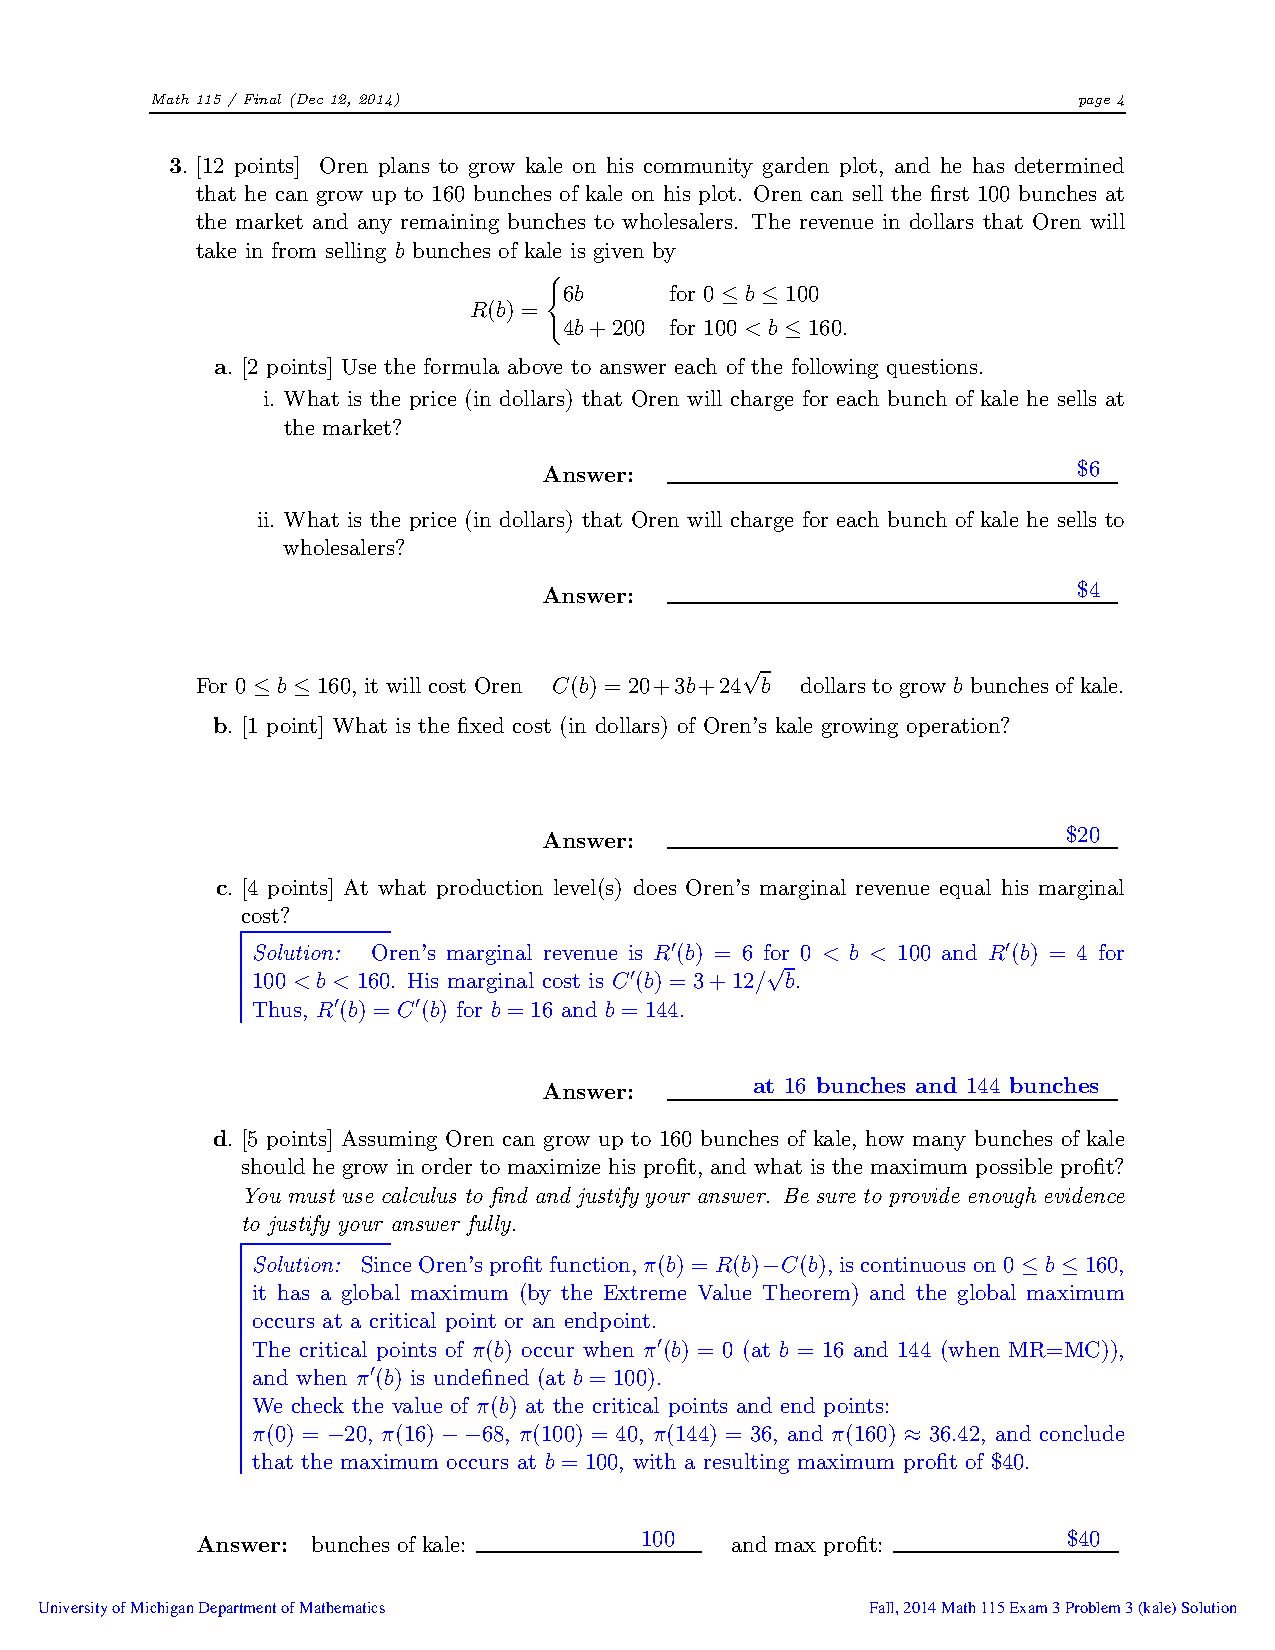
\includepdf[pages=-,pagecommand={}]{Figures/ExamProblemSolution.pdf}
    \else
    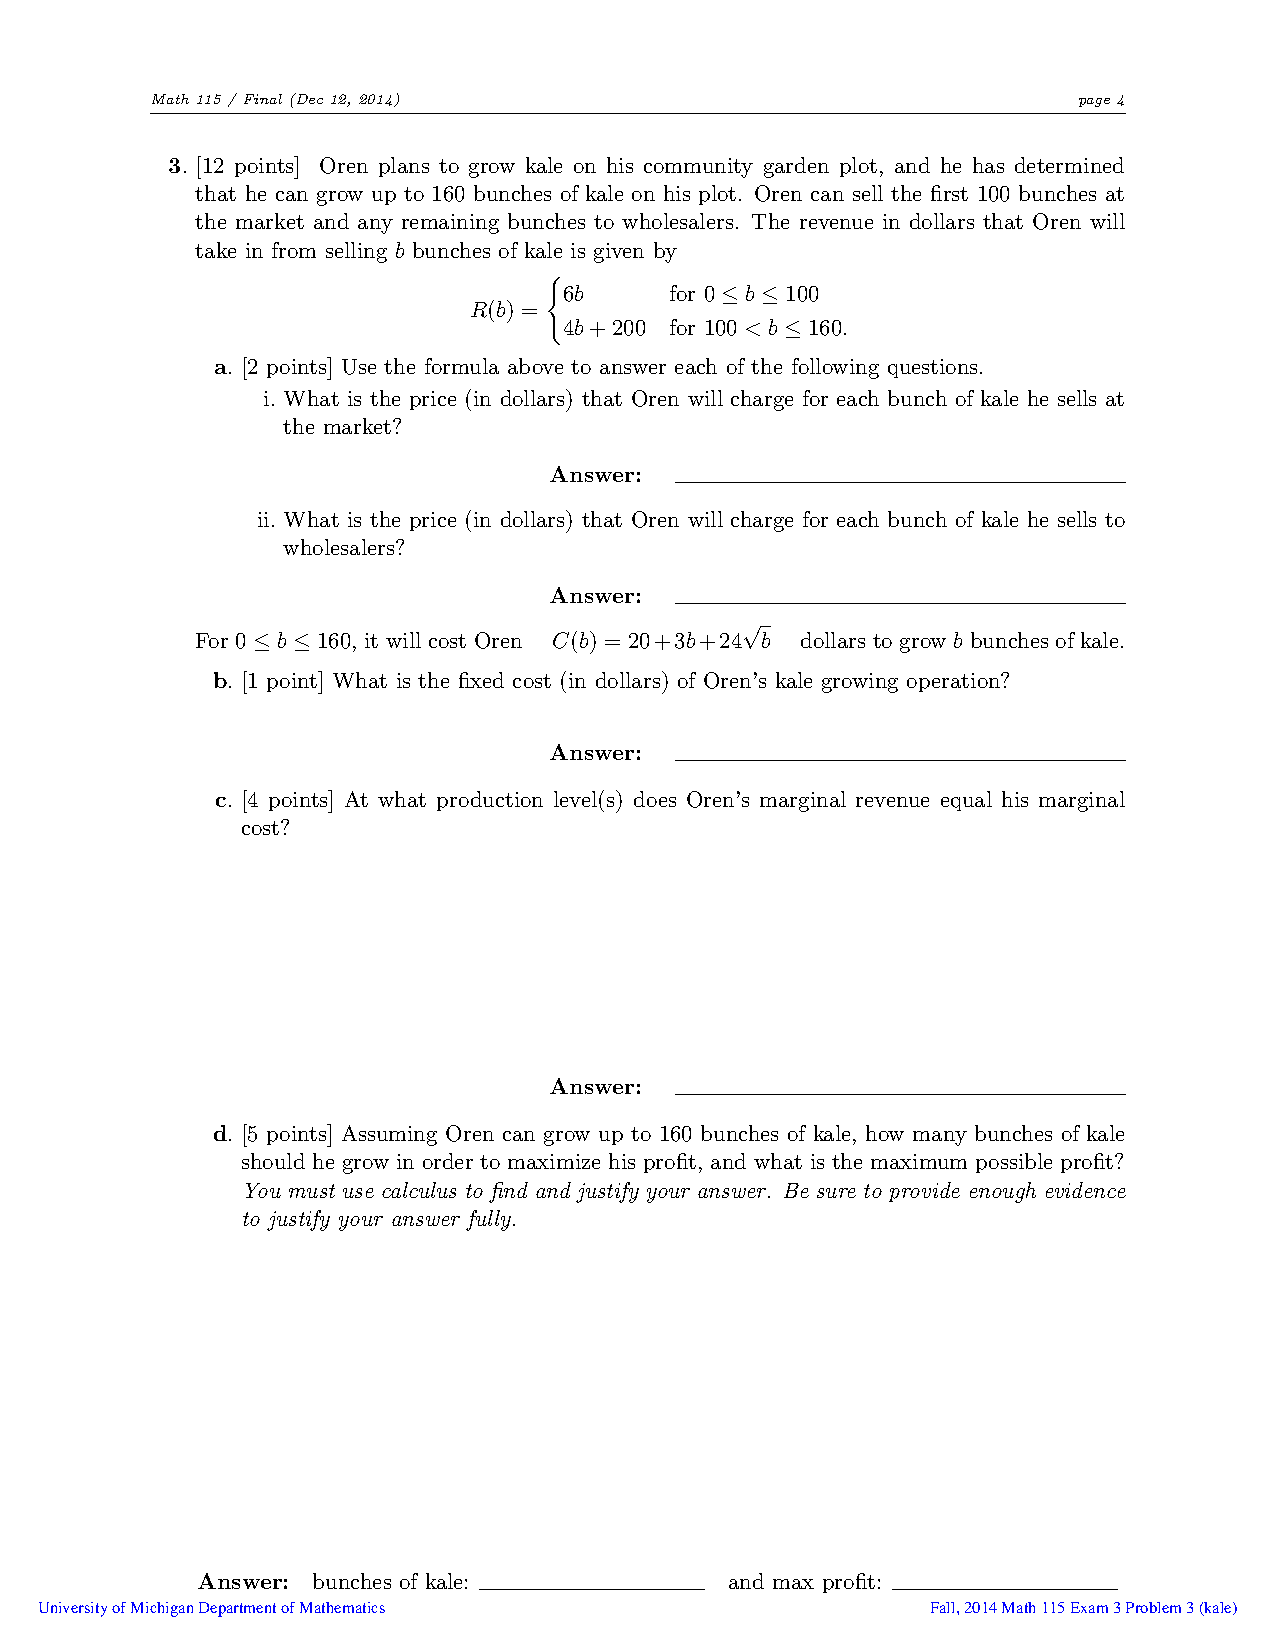
\includepdf[pages=-,pagecommand={}]{Figures/ExamProblem.pdf}
    \fi
    \pagebreak
  \question (Winter 2017 Final Exam) % problem 10
    The Happy Hives Bee Farm sells honey. The graph below shows marginal revenue
MR (dashed) and marginal cost MC (solid), in dollars per pound, where $h$ is the number of
pounds of honey.
\begin{center}
  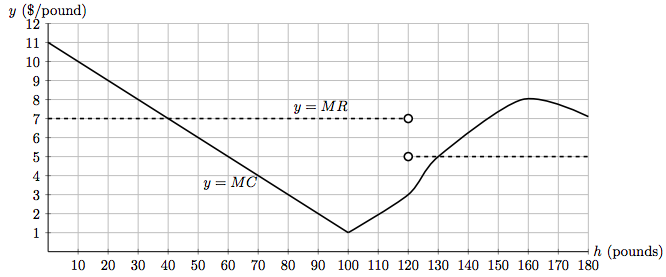
\includegraphics[scale=0.5]{Figures/bees}
\end{center}
Use the graph to estimate the answers to the following questions. If an answer can't be found with the information given, write \emph{NEI}.
	\begin{enumerate}[(i)]
		\item For what value(s) of $h$ in the interval $[0, 180]$ is the cost function $C$ minimized?
		\item For what value(s) of $h$ in the interval $[0, 180]$ is MC minimized?
		\item For what value(s) of h in the interval $[0, 180]$ is profit maximized?
		\item What are the fixed costs of the farm?
		\item For what values of $h$ in the interval $[0, 180]$ is the profit function concave up?
	\end{enumerate}
        \begin{solution}
         See \href{https://dhsp.math.lsa.umich.edu/exams/115exam3/w17/s10.pdf}{https://dhsp.math.lsa.umich.edu/exams/115exam3/w17/s10.pdf}
        \end{solution}

% 	{\bf Warning}: we do not know how to answer the following question yet, but we will soon!
% 	\item The farm currently sells 20 pounds of honey but is thinking of increasing to 80
% pounds of honey. Will this increase or decrease profit? By approximately how much will the profit change?
      \question (Fall 2016 Final Exam) % problem 10
        Yukiko has a small orchard where she grows Michigan apples. After careful study last season, Yukiko found that the total cost, in dollars, of producing a bushels of apples can
be modeled by
$$C(a) = -25500+26000e^{0.002a} \qquad \textrm{for } 0 \leqslant a \leqslant 320.$$
Qabil has promised to buy up to 100 bushels of apples for his famous apple ice cream. If Yukiko has any remaining apples, she has an agreement to sell them to Xanthippe’s cider mill at a reduced price. Let $R(a)$ be the revenue generated from selling a bushels of apples. Then
$$R(a)=\left\lbrace \begin{array}{ll} 70a & \textrm{for } 0 \leqslant a < 100 \\ 200+50a & \textrm{for } 100 < a \leqslant 320 \end{array}\right.$$
\begin{enumerate}[(a)]
	\item How much will Xanthippe's cider mill pay per bushel?
	\item What is Yukiko's fixed cost?
	\item For what quantities of bushels of apples sold would Yukiko's marginal revenue equal her marginal cost? Write none if appropriate.
	\item Assuming Yukiko can produce up to 320 bushels of apples, how many bushels should she produce in order to maximize her profit, and what would that maximum profit be? You must use calculus to find and justify your answer. Make sure to provide
enough evidence to justify your answer fully.
\end{enumerate}
\begin{solution}
  See \href{https://dhsp.math.lsa.umich.edu/exams/115exam3/f16/s10.pdf}{https://dhsp.math.lsa.umich.edu/exams/115exam3/f16/s10.pdf}
\end{solution}
\question (Fall 2017 Final Exam) % problem 2
	Jane has a company that produces a protein powder for an energy shake. The cost, in dollars, of producing $m$ pounds of protein powder is given by the function
	$$C(m)=\left\lbrace \begin{array}{ll} \frac{1}{4} (m+2)^2+8 & \textrm{for } 0 \leqslant m < 16 \\ 2m+57 & \textrm{for } 16 \leqslant m \leqslant 30 \end{array}\right.$$
	
	The revenue, in dollars, of selling m pounds of protein powder is given by
	$$R(m)=5m.$$
	
	\begin{enumerate}[(a)]
		\item What is the price, in dollars, at which Jane sells each pound of the protein powder?
		\item What is the fixed cost, in dollars, of producing Jane's protein powder?
		\item Find all values of $16 \leqslant m \leqslant 30$ for which Jane's profit is positive.
		\item Find all the values of $0 \leqslant m \leqslant 30$ where the marginal cost is equal to the marginal revenue for the protein powder. Show all your work to justify your answer.
		\item What is the maximum profit that Jane can make if she sells at most 30 pounds of protein powder? Use calculus to find and justify your answer, and make sure to provide enough evidence to fully justify your answer.
		\end{enumerate}
                \begin{solution}
                  See \href{https://dhsp.math.lsa.umich.edu/exams/115exam3/f17/s2.pdf}{https://dhsp.math.lsa.umich.edu/exams/115exam3/f17/s2.pdf}
                \end{solution}
\question (Fall 2013 Final Exam) % problem 2
Link has started a business selling winter clothes for cats. Among his most successful products are his new kitten mittens. He is currently selling his mittens for \$7 per set. Below is a graph of Link's marginal cost MC(q) and marginal revenue MR(q), in dollars per set of mittens, if he makes q sets of mittens this winter. Due to a shortage of yarn, Link can make a maximum of 200 sets of mittens this winter. In order to start making mittens, Link must spend \$40 on knitting supplies (in other words, it costs \$40 to make 0 sets of mittens).	
\begin{center}
  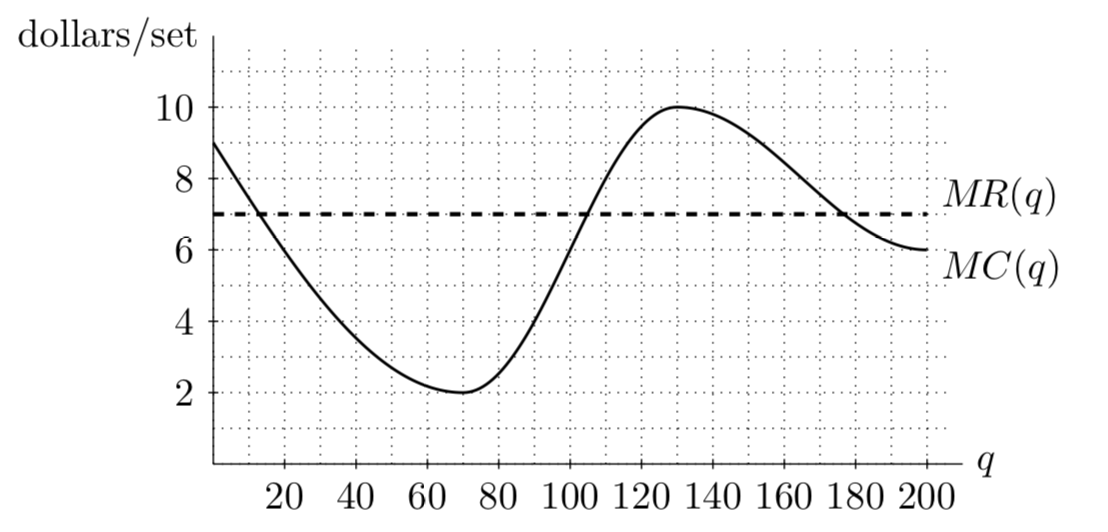
\includegraphics[scale=0.5]{Figures/link}
\end{center}
\begin{enumerate}[(a)]
	\item Approximately how many sets of mittens should Link make this winter in order to maximize his profit?
	
	{\bf Warning}: we do not know how to answer the following question yet, but we will soon!
	\item If the price per set is raised to \$9, approximately how many sets of mittens should Link make in order to maximize his profit?
	\item Link makes a deal with a store that would like to buy his cat hats. If the store buys up to 50 hats, then each one will cost \$10. If the store buys more than 50 hats, then Link will reduce the price of the entire order by \$0.05 per hat for every additional hat over 50. (For example, if the store buys 52 hats, they will pay \$9.90 per hat.) Write a formula for a function L(q) which gives Link's revenue if he sells q hats to the store.
\end{enumerate}
\begin{solution}
  See \href{https://dhsp.math.lsa.umich.edu/exams/115exam3/f13/s2.pdf}{https://dhsp.math.lsa.umich.edu/exams/115exam3/f13/s2.pdf}
\end{solution}
\end{questions}
\end{document}
%%% Local Variables:
%%% mode: latex
%%% TeX-master: t
%%% End:
